%\documentclass[handout]{beamer}
\documentclass[presentation]{beamer}
\usepackage[utf8]{inputenc}
\usepackage{amsmath, pdfpages, pdflscape, lscape, color, listings, hyperref, amssymb, graphicx,textcomp,varioref, afterpage, subcaption, float, bm, tikz, colortbl}

\global
\newcommand{\Fig}[1]{Figure \ref{#1}}
\newcommand{\fig}[1]{figure \ref{#1}}
\newcommand{\tab}[1]{table \ref{#1}}
\newcommand{\eq}[1]{equation \ref{#1}}
\newcommand{\Eq}[1]{Equation \ref{#1}}
\newcommand{\alg}[1]{algorithm \ref{#1}}
\newcommand{\Alg}[1]{Algorithm \ref{#1}}
\newcommand{\chp}[1]{chapter  \ref{#1}}
\newcommand{\Chp}[1]{Chapter  \ref{#1}}
\newcommand{\e}[1]{\cdot 10^{#1}}
\newcommand{\h}{\hbar}
\newcommand{\der}[2]{\frac{\partial #1}{\partial #2}}
\newcommand{\dder}[2]{\frac{\partial^2 #1}{\partial #2^2}}
\newcommand{\p}{\boldsymbol{P}}
\newcommand{\q}{\boldsymbol{q}}
\newcommand{\norm}[1]{\left\lVert#1\right\rVert_{\!Q}}
\newcommand{\inner}[1]{\left\langle#1\right\rangle_{\!Q}}
\newcommand{\coef}[2]{\frac{\inner{#1,#2}}{\norm{#2}^2}}

\newcommand{\gooditem}[1]{\setbeamercolor{item}{fg=green}\item #1}
\newcommand{\baditem}[1]{\setbeamercolor{item}{fg=red}\item #1}

\DeclareMathOperator*{\argmin}{argmin}
\DeclareMathOperator*{\argmax}{argmax}

\newcommand{\E}[1]{\mbox{E}\!\left(#1\right)}
\newcommand{\Var}[1]{\mbox{Var}\!\left(#1\right)}
\newcommand{\Cov}[1]{\mbox{Cov}\!\left(#1\right)}



\setbeamertemplate{blocks}[rounded][shadow=false]


\usefonttheme[onlysmall]{structurebold}
% Use a bold face title font
\setbeamerfont{title}{series=\bfseries}
\setbeamerfont{frametitle}{series=\bfseries}

% This is not created yet, but should be...
%\usecolortheme{simula}

% Suppress navigation symbols
\setbeamertemplate{navigation symbols}{}

\definecolor{listingsstringcolor}{rgb}{0,0.5,0}
\definecolor{listingskeywordcolor}{rgb}{0,0,1}
\definecolor{listingsbasiccolor}{rgb}{0.0,0.0,0.0}

\definecolor{myred}{RGB}{190,0,0}

 \newcommand{\listingsfont}{\sffamily}

 \lstset{
    language=python,
    commentstyle=\color{red},
     basicstyle=\color{listingsbasiccolor},
    keywordstyle=\color{listingskeywordcolor},
    stringstyle=\color{listingsstringcolor},
 tabsize=4,                       % sets default tabsize to 2 spaces
 morekeywords={as, assert, with, yield},
escapeinside={||},
basicstyle=\ttfamily\footnotesize,
columns=fixed
}

\newenvironment{chaospy}[1]
{\color{gray!30!black}
     \usebackgroundtemplate{
   \begin{tikzpicture}[remember picture, overlay]
     \node[anchor = center, opacity=.15] (image) at (current page.center) {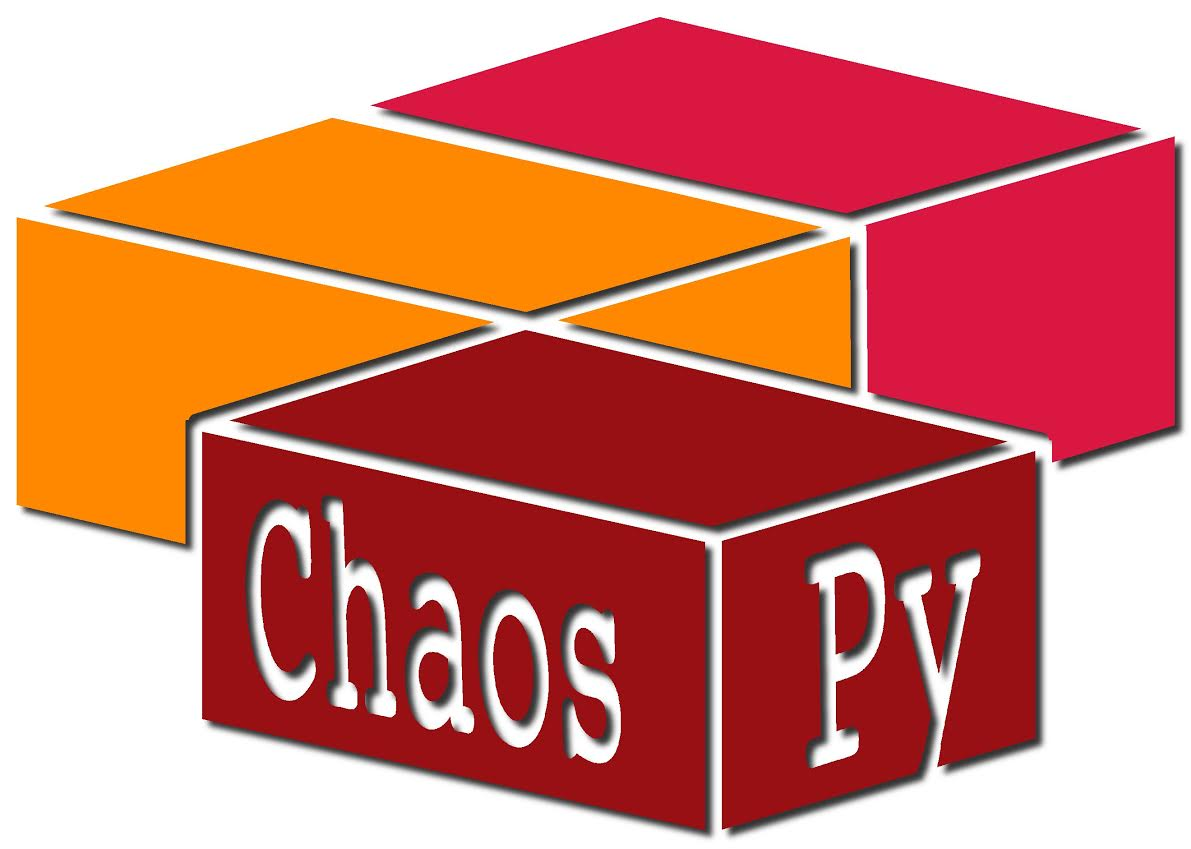
\includegraphics[scale=0.25]{chaospy_logo.jpg}};
   \end{tikzpicture}}
     \begin{frame}[fragile, environment=chaospy]
    \frametitle{{#1}}}
{\end{frame}}


\definecolor{keywords}{RGB}{255,0,90}
\definecolor{comments}{RGB}{0,0,113}
\definecolor{red}{RGB}{160,0,0}
\definecolor{green}{RGB}{0,150,0}


\setbeamercolor{title}{fg=myred}
\setbeamercolor{frametitle}{fg=black!65!white,bg=white}
\setbeamercolor{normal text}{fg=black!75!white,bg=white}
\setbeamercolor{structure}{fg=black,bg=white}



\graphicspath{{./figures/}}


\title{Chaospy: \\ A modular implementation of Polynomial Chaos expansions and Monte Carlo methods}
\author{Simen Tennøe\\ \vspace{5mm}\footnotesize Supervisors:\\ \vspace{0.5mm} Jonathan Feinberg, Hans Petter Langtangen, Gaute Einevoll and Geir Halnes}
\institute{University of Oslo, CINPLA}
\date{}
 % \titlegraphic{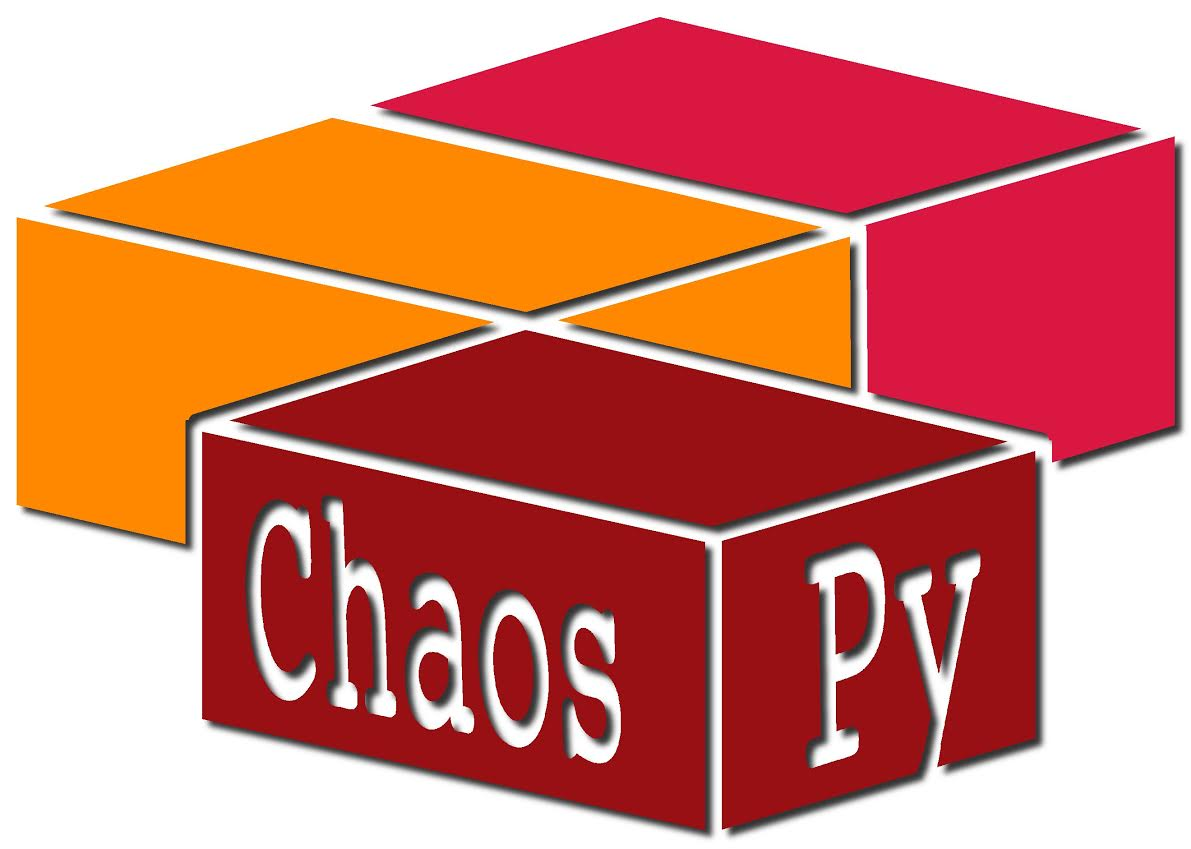
\includegraphics[width=\textwidth]{chaospy_logo.jpg}}

\begin{document}

% \maketitle

% \begin{frame}
%    \begin{tikzpicture}[remember picture, overlay]
%      \node[anchor = center, opacity=.25] (image) at (current page.center) {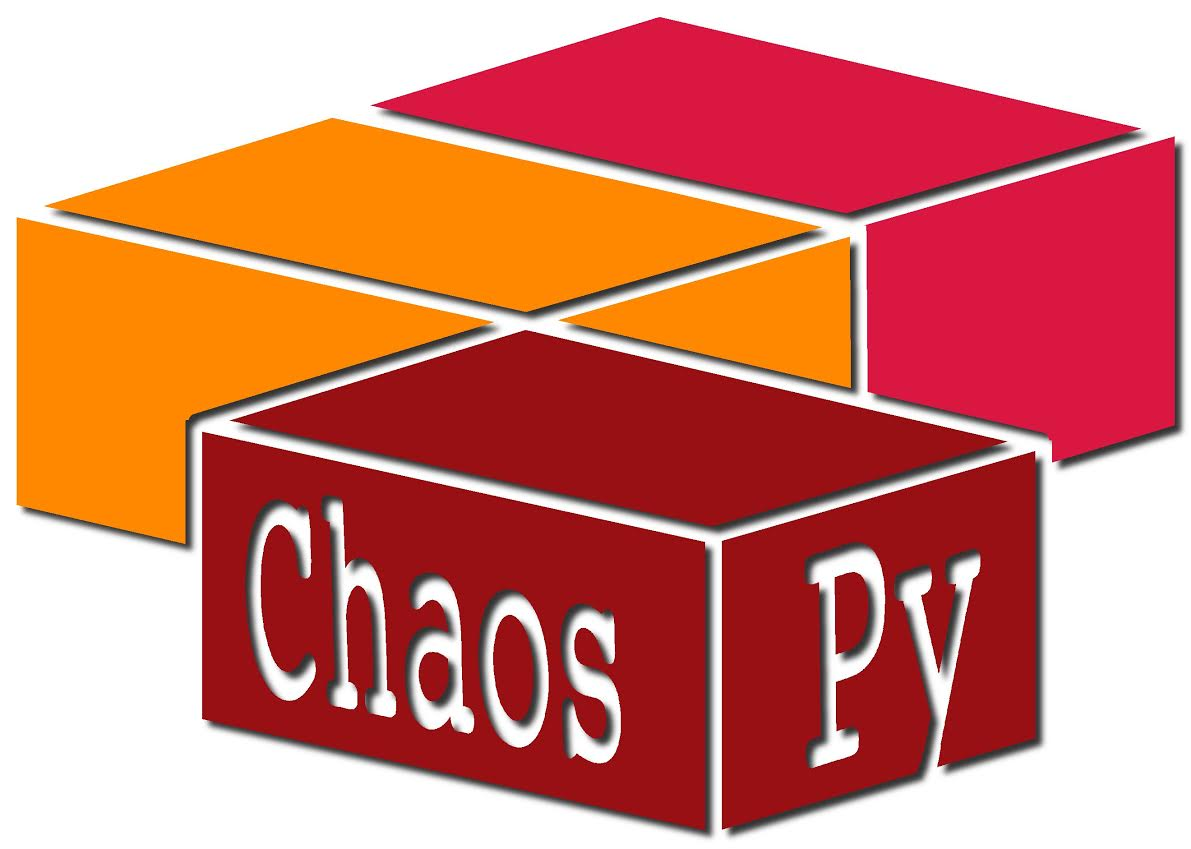
\includegraphics[scale=0.25]{chaospy_logo.jpg}};
%    \end{tikzpicture}
%
% \begin{center}
%     \textbf{ \color{myred} \Large Chaospy: \\ \vspace{1mm} A modular implementation of polynomial\\ \vspace{1mm} chaos expansions and Monte Carlo methods}
% \end{center}
% \begin{center}
%      \large \vspace{5mm} Simen Tennøe\\ \vspace{5mm}\footnotesize Supervisors:\\ \vspace{0.5mm} Jonathan Feinberg, Hans Petter Langtangen, Gaute Einevoll and Geir Halnes
% \end{center}
%
% \begin{center}
%     \small University of Oslo, CINPLA
% \end{center}
% %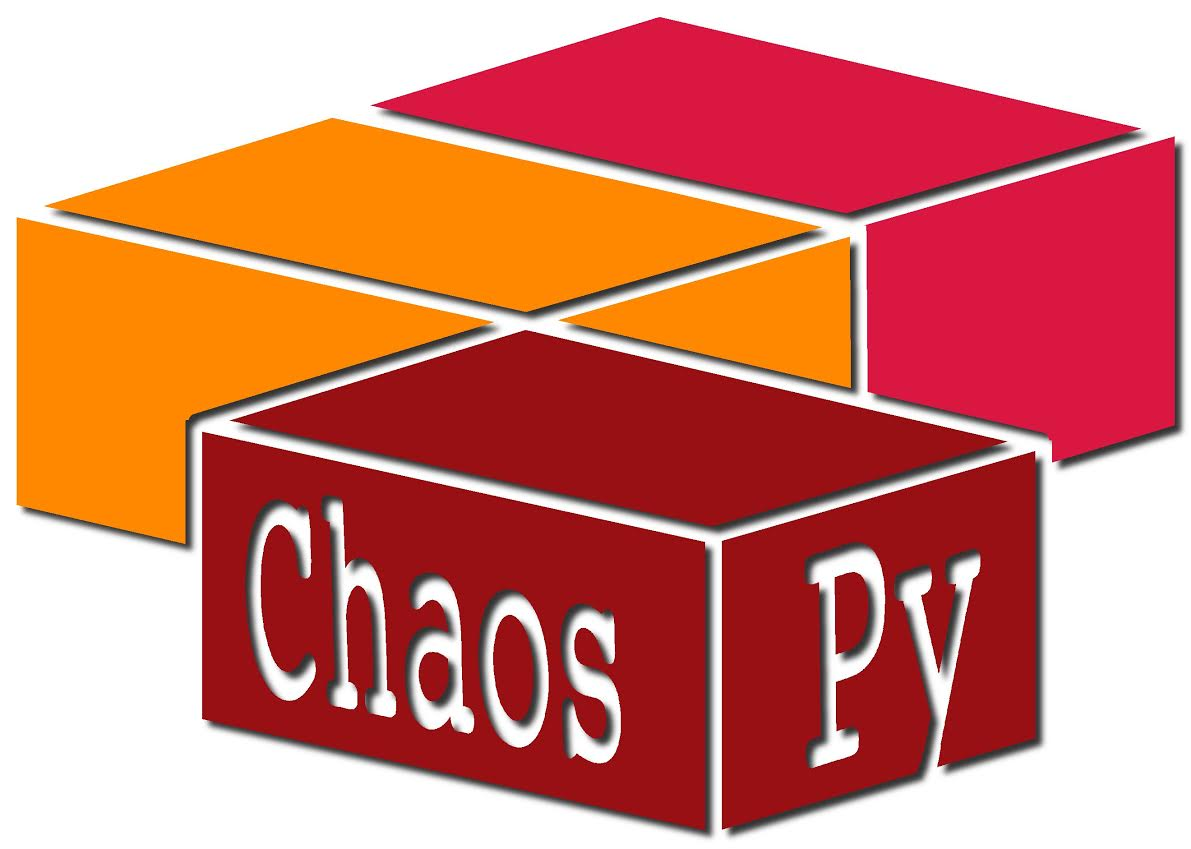
\includegraphics[width=\textwidth]{chaospy_logo.jpg}
%
% \end{frame}




\begin{frame}
\begin{center}
    \textbf{\color{myred}\Large Chaospy: \\ \vspace{1mm} A modular implementation of Polynomial\\ \vspace{1mm} Chaos expansions and Monte Carlo methods}
\end{center}

% \frametitle{\textbf{\color{myred}\Large Chaospy: \\ \vspace{1mm} A modular implementation of polynomial\\ \vspace{1mm} chaos expansions and Monte Carlo methods}}

     \large \vspace{8mm} Simen Tennøe

      \vspace{6mm}
      \footnotesize Supervisors:

    %
      \vspace{1mm}
      Jonathan Feinberg

      Hans Petter Langtangen

      Gaute Einevoll

      Geir Halnes

      \vspace{5mm}
    \small University of Oslo, CINPLA

 \begin{tikzpicture}[remember picture,overlay]
    \node [xshift=0.2\paperwidth,yshift=-0.14\paperheight] at (current page.center)
          {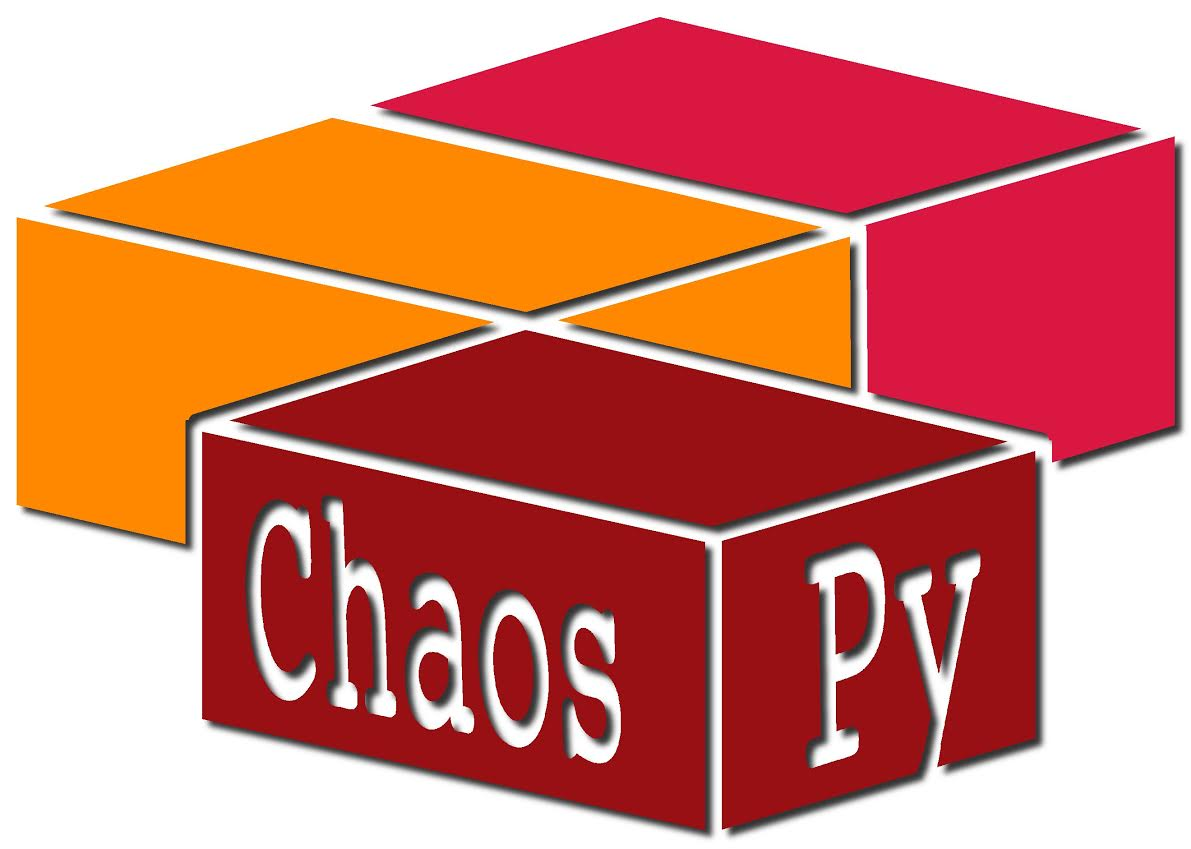
\includegraphics[width = 0.5\paperwidth ]{chaospy_logo.jpg}};
  \end{tikzpicture}

  \begin{tikzpicture}[remember picture,overlay]
    \node [xshift=1.35cm,yshift=0.55cm] at (current page.south west)
          {
\includegraphics[width = 0.2\paperwidth ]{cinpla.png}};
  \end{tikzpicture}

\end{frame}




\begin{frame}[fragile]{Chaospy is a Python toolbox for forward model UQ}


    \begin{tikzpicture}[remember picture, overlay, font=\sffamily]
      \node [align=left, xshift=-0.4\textwidth,yshift=0.15\textwidth] (image3) at (current page.center)
            {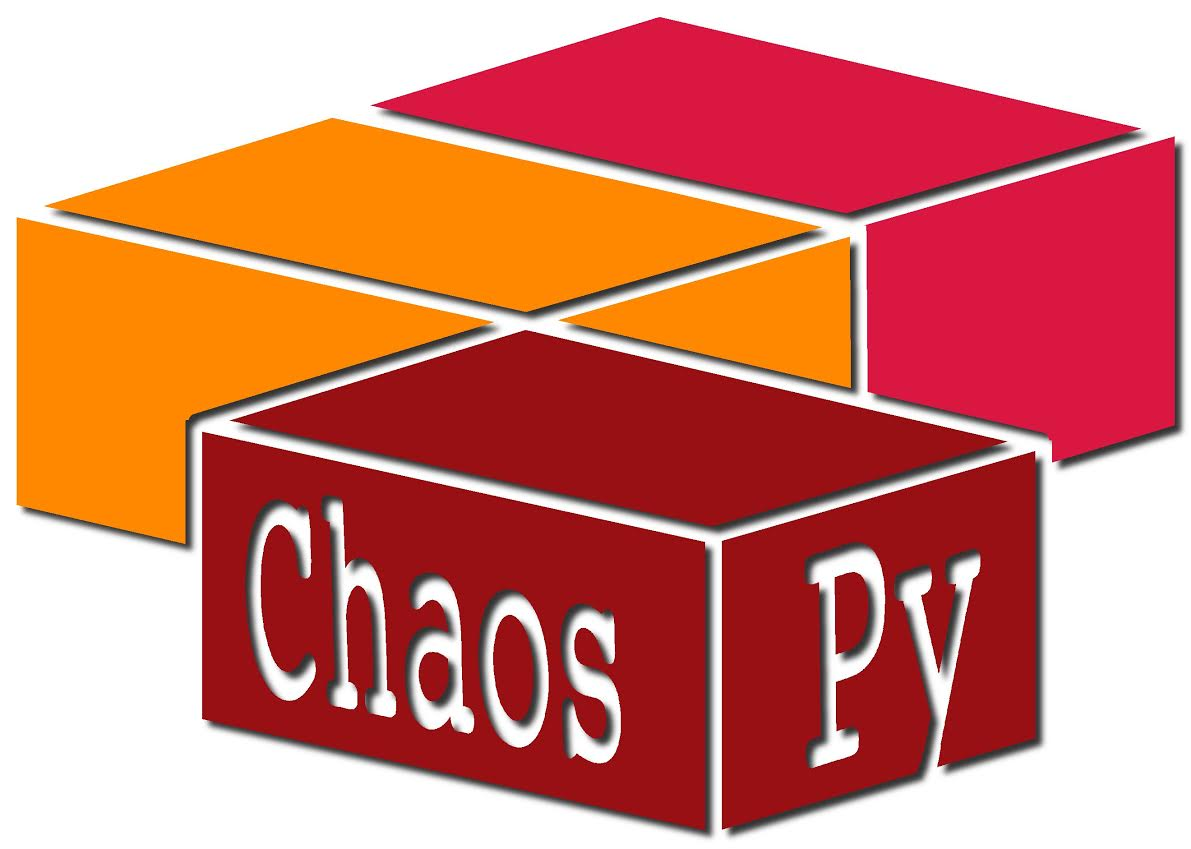
\includegraphics[width = 0.2\textwidth]{chaospy_logo.jpg}};
      \node[align=left] at (image3.east) {\hspace{5cm} \bf Properties of Chaospy};
    \end{tikzpicture}

  \pause

  \begin{tikzpicture}[remember picture, overlay, font=\sffamily]
  \node [align=left, xshift=-0.2\textwidth,yshift=-0.05\textwidth] (image1) at (current page.center)
      {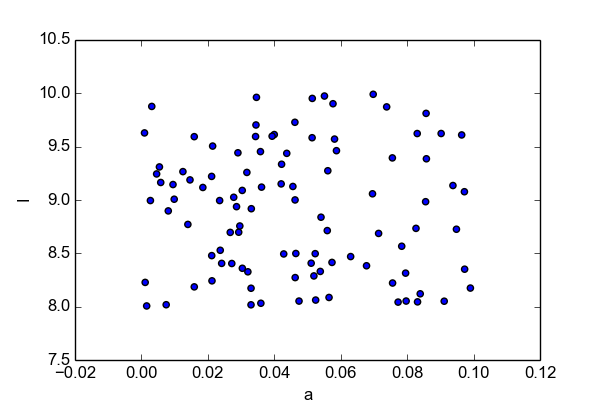
\includegraphics[width = 0.25\textwidth]{samples.png}};
  \node[align=left] at (image1.east) {\hspace{4.5cm} \bf Monte Carlo methods};
  \end{tikzpicture}

\pause


    \begin{tikzpicture}[remember picture, overlay, font=\sffamily]
      \node [align=left, xshift=0\textwidth,yshift=-0.25\textwidth] (image2) at (current page.center)
            {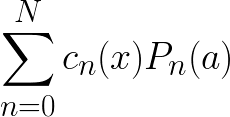
\includegraphics[width = 0.25\textwidth]{pc.png}};
      \node[align=left] at (image2.east) {\hspace{4cm} \bf Polynomial Chaos};
    \end{tikzpicture}

\end{frame}



\begin{frame}{What is new in Chaospy}

\vspace{-7mm}
\begin{columns}

     \column{.5\textwidth}
     \begin{center}
      \textbf<1>{Chaospy is modular and therefore very flexible}
     \end{center}
     \column{.5\textwidth}
     \begin{center}
            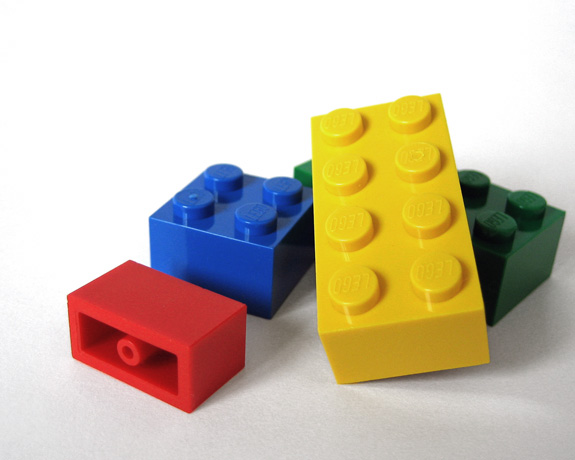
\includegraphics[width=0.5\textwidth]{lego.jpg}
     \end{center}

 \end{columns}

\pause
\vspace{7mm}
\begin{columns}
     \column{.5\textwidth}
     \begin{center}
            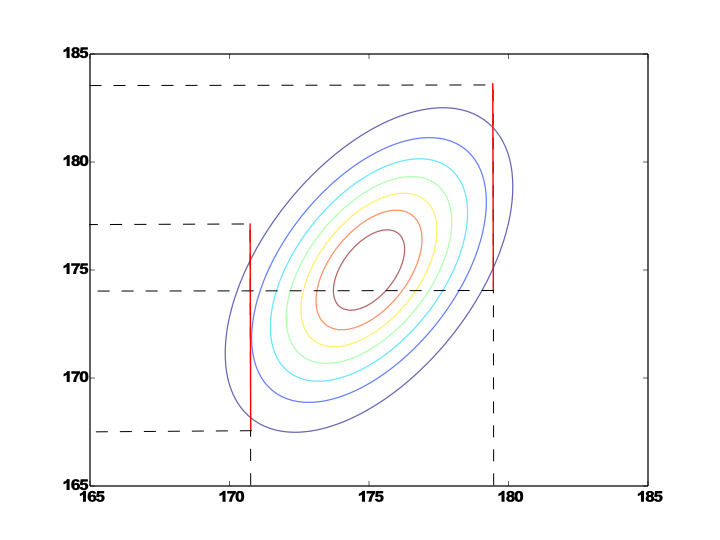
\includegraphics[width=0.5\textwidth]{dependent.png}
     \end{center}
     \column{.5\textwidth}
     \begin{center}
      \textbf<2>{Chaospy has support for dependent variables}
     \end{center}
 \end{columns}

\pause
\vspace{7mm}
 \begin{columns}
      \column{.5\textwidth}
      \begin{center}
             \textbf<3>{Chaospy has a large collection of methods and distributions}
      \end{center}
      \column{.5\textwidth}
      \begin{center}
      \pause \textbf<4>{It is easy to compare different methods on given a problem}
      \end{center}
  \end{columns}

\end{frame}



\begin{frame}
  \frametitle{Comparing Chaospy with Turns and Dakota}

\begin{center}
\newcolumntype{g}{>{\columncolor{gray}}l}
\def\arraystretch{1.1}
  \begin{tabular}{ll|lll}
  Feature	&    & Dakota &	Turns	& Chaospy\\\hline
  Distributions	&& 11	& 26	& \textbf<3>{\textcolor<3>{green}{64}}\\
  Copulas	&& 1	& 7	& \textbf<2->{\textcolor<2->{red}6}\\
  Sampling schemes &	& 4	& 7.5	& \textbf<2->{\textcolor<2->{red}7}\\
  Orthogonal polynomial schemes &	& 4	& 3	& \textbf<3>{\textcolor<3>{green}5}\\
  Numerical integration strategies &	& 7	& 0	& \textbf<3>{\textcolor<3>{green}7}\\
  Regression methods &	& 5 & 	4	& \textbf<3>{\textcolor<3>{green}8}\\
  Analytical metrics &	& 6	& 6	& \textbf<3>{\textcolor<3>{green}7}\\
\end{tabular}
\end{center}
\end{frame}
%--- Next Frame ---%




\begin{frame}{Chaospy has support for many different methods}

  \begin{itemize}[<+->]
    \setlength{\itemsep}{5pt}
    \item Monte Carlo with variance reduction techniques
    \item Intrusive and non-intrusive polynomial chaos
    \begin{itemize}
        \vspace{5pt}
        \setlength{\itemsep}{5pt}
        \item Pseudo-spectral method
        \item Point collocation/regression
    \end{itemize}
  \end{itemize}

\end{frame}



\begin{chaospy}{All Chaospy needs is a Python wrapper around the forward model}
\begin{lstlisting}[language=python]
def solver(*node):
    # node: tuple of the uncertain stochastic parameters

    model.set_parameters(node)
    |\pause|
    model.run()
    |\pause|
    results = model.post_processing()
    |\pause|
    return results

\end{lstlisting}

\end{chaospy}


\begin{frame}
 \frametitle{Chaospy is a completly generic software; for simplicity we use a very simple example problem}
 \vspace{-10mm}
  \begin{align*}
    \frac{d u(x)}{dx} & =-au(x),\qquad u(0) = I.
  \end{align*}
  \vspace{-5 mm}
  \begin{itemize}
    \item[$u$] The quantity of interest.
    \item[$x$] Spatial location.
    \item[$a,I$] Parameters containing uncertainties.
  \end{itemize}

%\vspace{-5 mm}
 \pause
%Initially assume model parameters:
\begin{align*}
a &\sim \text{Uniform(0, 0.1)} & I& \sim \text{Uniform(8, 10)}
\end{align*}
\pause
\vspace{5 mm}
%Analytical solution
%\[u(x; a, I) = Ie^{-ax}.\]

%\pause
%\vspace{5mm}
We want to compute E(u) and Var(u).

\end{frame}





\begin{frame}[fragile]
{Monte Carlo integration can be used for any model}

    \begin{figure}
    
\includegraphics[width=\textwidth]{MC.png}
  \end{figure}
\end{frame}

%
% \begin{chaospy}{Creating multivariate probability distributions in Chaospy}
% \begin{lstlisting}[language=python]
% dist_a = cp.Uniform(0, 0.1)
% dist_I = cp.Uniform(8, 10)
% |\pause|
% dist = cp.J(dist_a, dist_I)
% \end{lstlisting}
% \end{chaospy}








\begin{chaospy}{Monte Carlo with Chaospy}
    \scriptsize
\begin{lstlisting}[language=python]
import chaospy as cp
import numpy as np
|\pause|
dist_a = cp.Uniform(0, 0.1)
dist_I = cp.Uniform(8, 10)
|\pause|
# Joint distribution
dist = cp.J(dist_a, dist_I)
|\pause|
samples = dist.sample(size=1000)
|\pause|
# solver returns the u(x), where x is fixed
samples_u = [solver(a, I) for a, I in samples]

# solver_u : list of all u values for each
#            set of uncertain parameters
|\pause|
E = np.mean(samples_u, 0)
Var = np.var(samples_u, 0)
\end{lstlisting}
\end{chaospy}


\begin{frame}
  \frametitle{Convergence of Monte Carlo is slow}
  \vspace{-4mm}
  \begin{align*}
      \varepsilon_E &= \int|\E{u} - \E{\hat{u}}|\,dx & \qquad
      \varepsilon_{Var} &= \int|\Var{u} - \Var{\hat{u}}|\,dx
  \end{align*}
  \vspace{-5mm}
\pause

  \begin{center}
    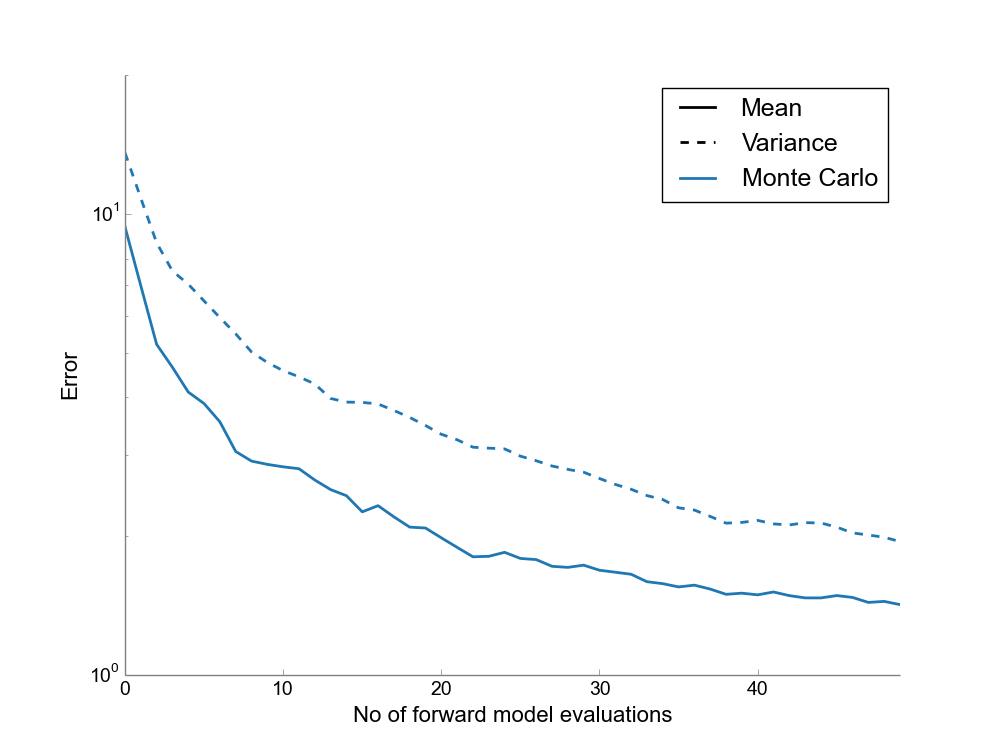
\includegraphics[width=0.9\textwidth]{MC_convergence_2D.png}
  \end{center}
\end{frame}



\begin{frame}[fragile]
 \frametitle{Chaospy has several variance reduction techniques for sampling a distribution}
 \vspace{-5mm}
 \begin{columns}
     \column{.5\textwidth}
     \begin{center}
                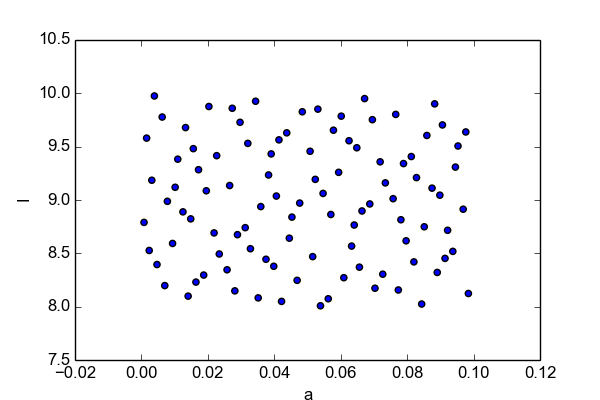
\includegraphics[width=0.65\textwidth]{samples_H.png}

                Hammersley sampling:

                \scriptsize
                \verb;nodes = dist.sample(100, "M");
                \normalsize
                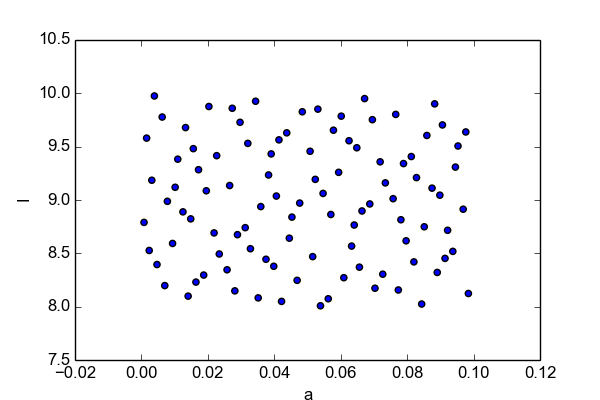
\includegraphics[width=0.65\textwidth]{samples_H.png}

                Halton sampling

                \scriptsize
                \verb;nodes = dist.sample(100, "H");
                \normalsize

     \end{center}
     \column{.5\textwidth}
     \begin{center}
                  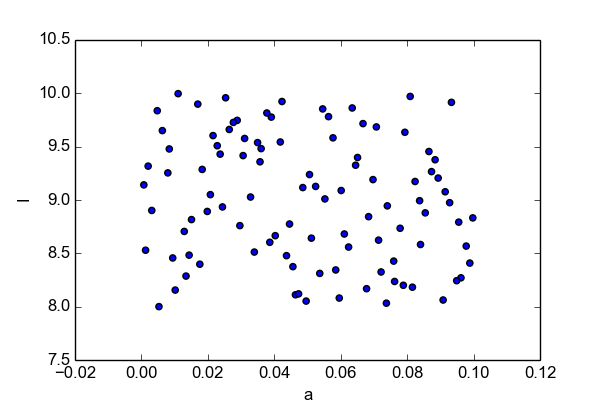
\includegraphics[width=0.65\textwidth]{samples_L.png}

                Latin Hypercube sampling:

                \scriptsize
                \verb;nodes = dist.sample(100, "L");
                \normalsize



                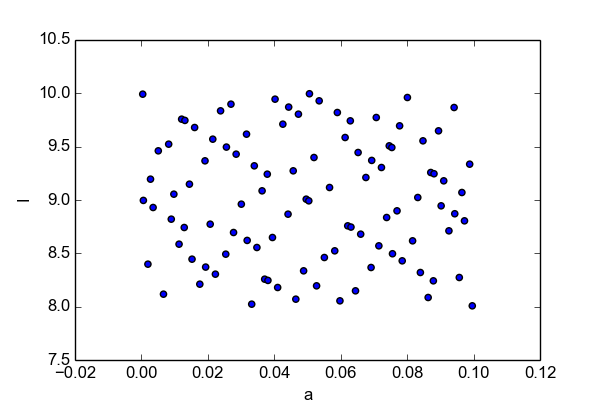
\includegraphics[width=0.65\textwidth]{samples_S.png}

                Sobol sampling

                \scriptsize
                \verb;nodes = dist.sample(100, "S");
                \normalsize
     \end{center}
 \end{columns}
\end{frame}



\begin{frame}
  \frametitle{The different sampling schemes available in Chaospy compared to Turns and Dakota}
\begin{center}
\def\arraystretch{1.1}

  \begin{tabular}{ll|lll}
        && Dakota &	Turns &	Chaospy\\
  Quasi-Monte Carlo scheme && & & \\\hline
  Faure sequence &&	No &	Yes &	\textbf{\textcolor{red}{No}}\\
  Halton sequence &&	Yes& 	Yes	& \textbf{\textcolor{green}{Yes}}\\
  Hammersley sequence &&	Yes &	Yes &	\textbf{\textcolor{green}{Yes}}\\
  Haselgrove sequence &&	No &	Yes	& \textbf{\textcolor{red}{No}}\\
  Korobov latice &&	No &	No&	\textbf{\textcolor{green}{Yes}}\\
  Niederreiter sequence &&	No&	Yes&	\textbf{\textcolor{red}{No}}\\
  Sobol sequence &&	No &	Yes &	\textbf{\textcolor{green}{Yes}}\\\\

  Other methods &&&&\\\hline
  Antithetic variables &&	No&	No&	\textbf{\textcolor{green}{Yes}}\\
  Importance sampling &&	Yes	&Yes&	\textbf{\textcolor{green}{Yes}}\\
  Latin Hypercube sampling &&	Yes &	Limited &	\textbf{\textcolor{green}{Yes}}\\
\end{tabular}
\end{center}
\end{frame}



\begin{chaospy}{Quasi-Monte Carlo with Latin Hypercube sampling}
    \scriptsize

\begin{lstlisting}[language=python]
import chaospy as cp
import numpy as np

dist_a = cp.Uniform(0, 0.1)
dist_I = cp.Uniform(8, 10)
dist = cp.J(dist_a, dist_I)

samples = dist.sample(size=1000|\only<2>{, \color{myred}{rule="L"}}|)

samples_u = [solver(a, I) for a, I in samples]

E = np.mean(samples_u, 0)
Var = np.var(samples_u, 0)
\end{lstlisting}
\end{chaospy}




\begin{frame}
  \frametitle{Convergence of quasi-Monte Carlo is better than Monte Carlo, but still slow}
\vspace{-5mm}
  \begin{center}
    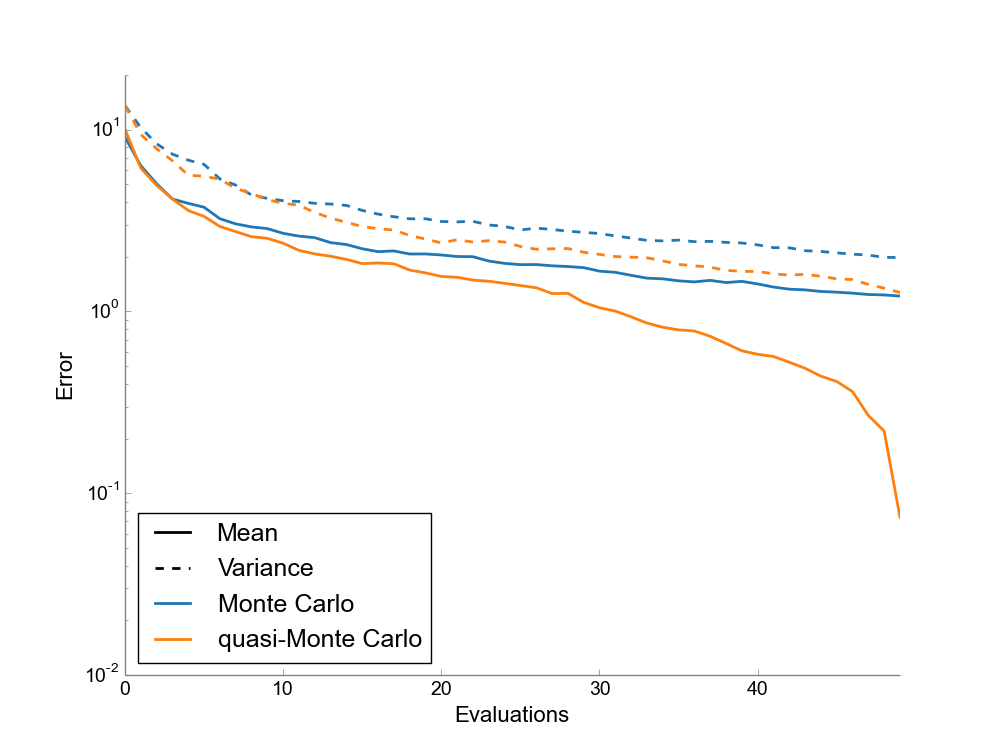
\includegraphics[width=1\textwidth]{qMC-MC_convergence_2D.png}
  \end{center}
\end{frame}



 %\begin{frame}
 %\frametitle{All random variables can with aid of the Rosenblatt transformations be transformed to/from the uniform distribution}
 %\begin{figure}
 %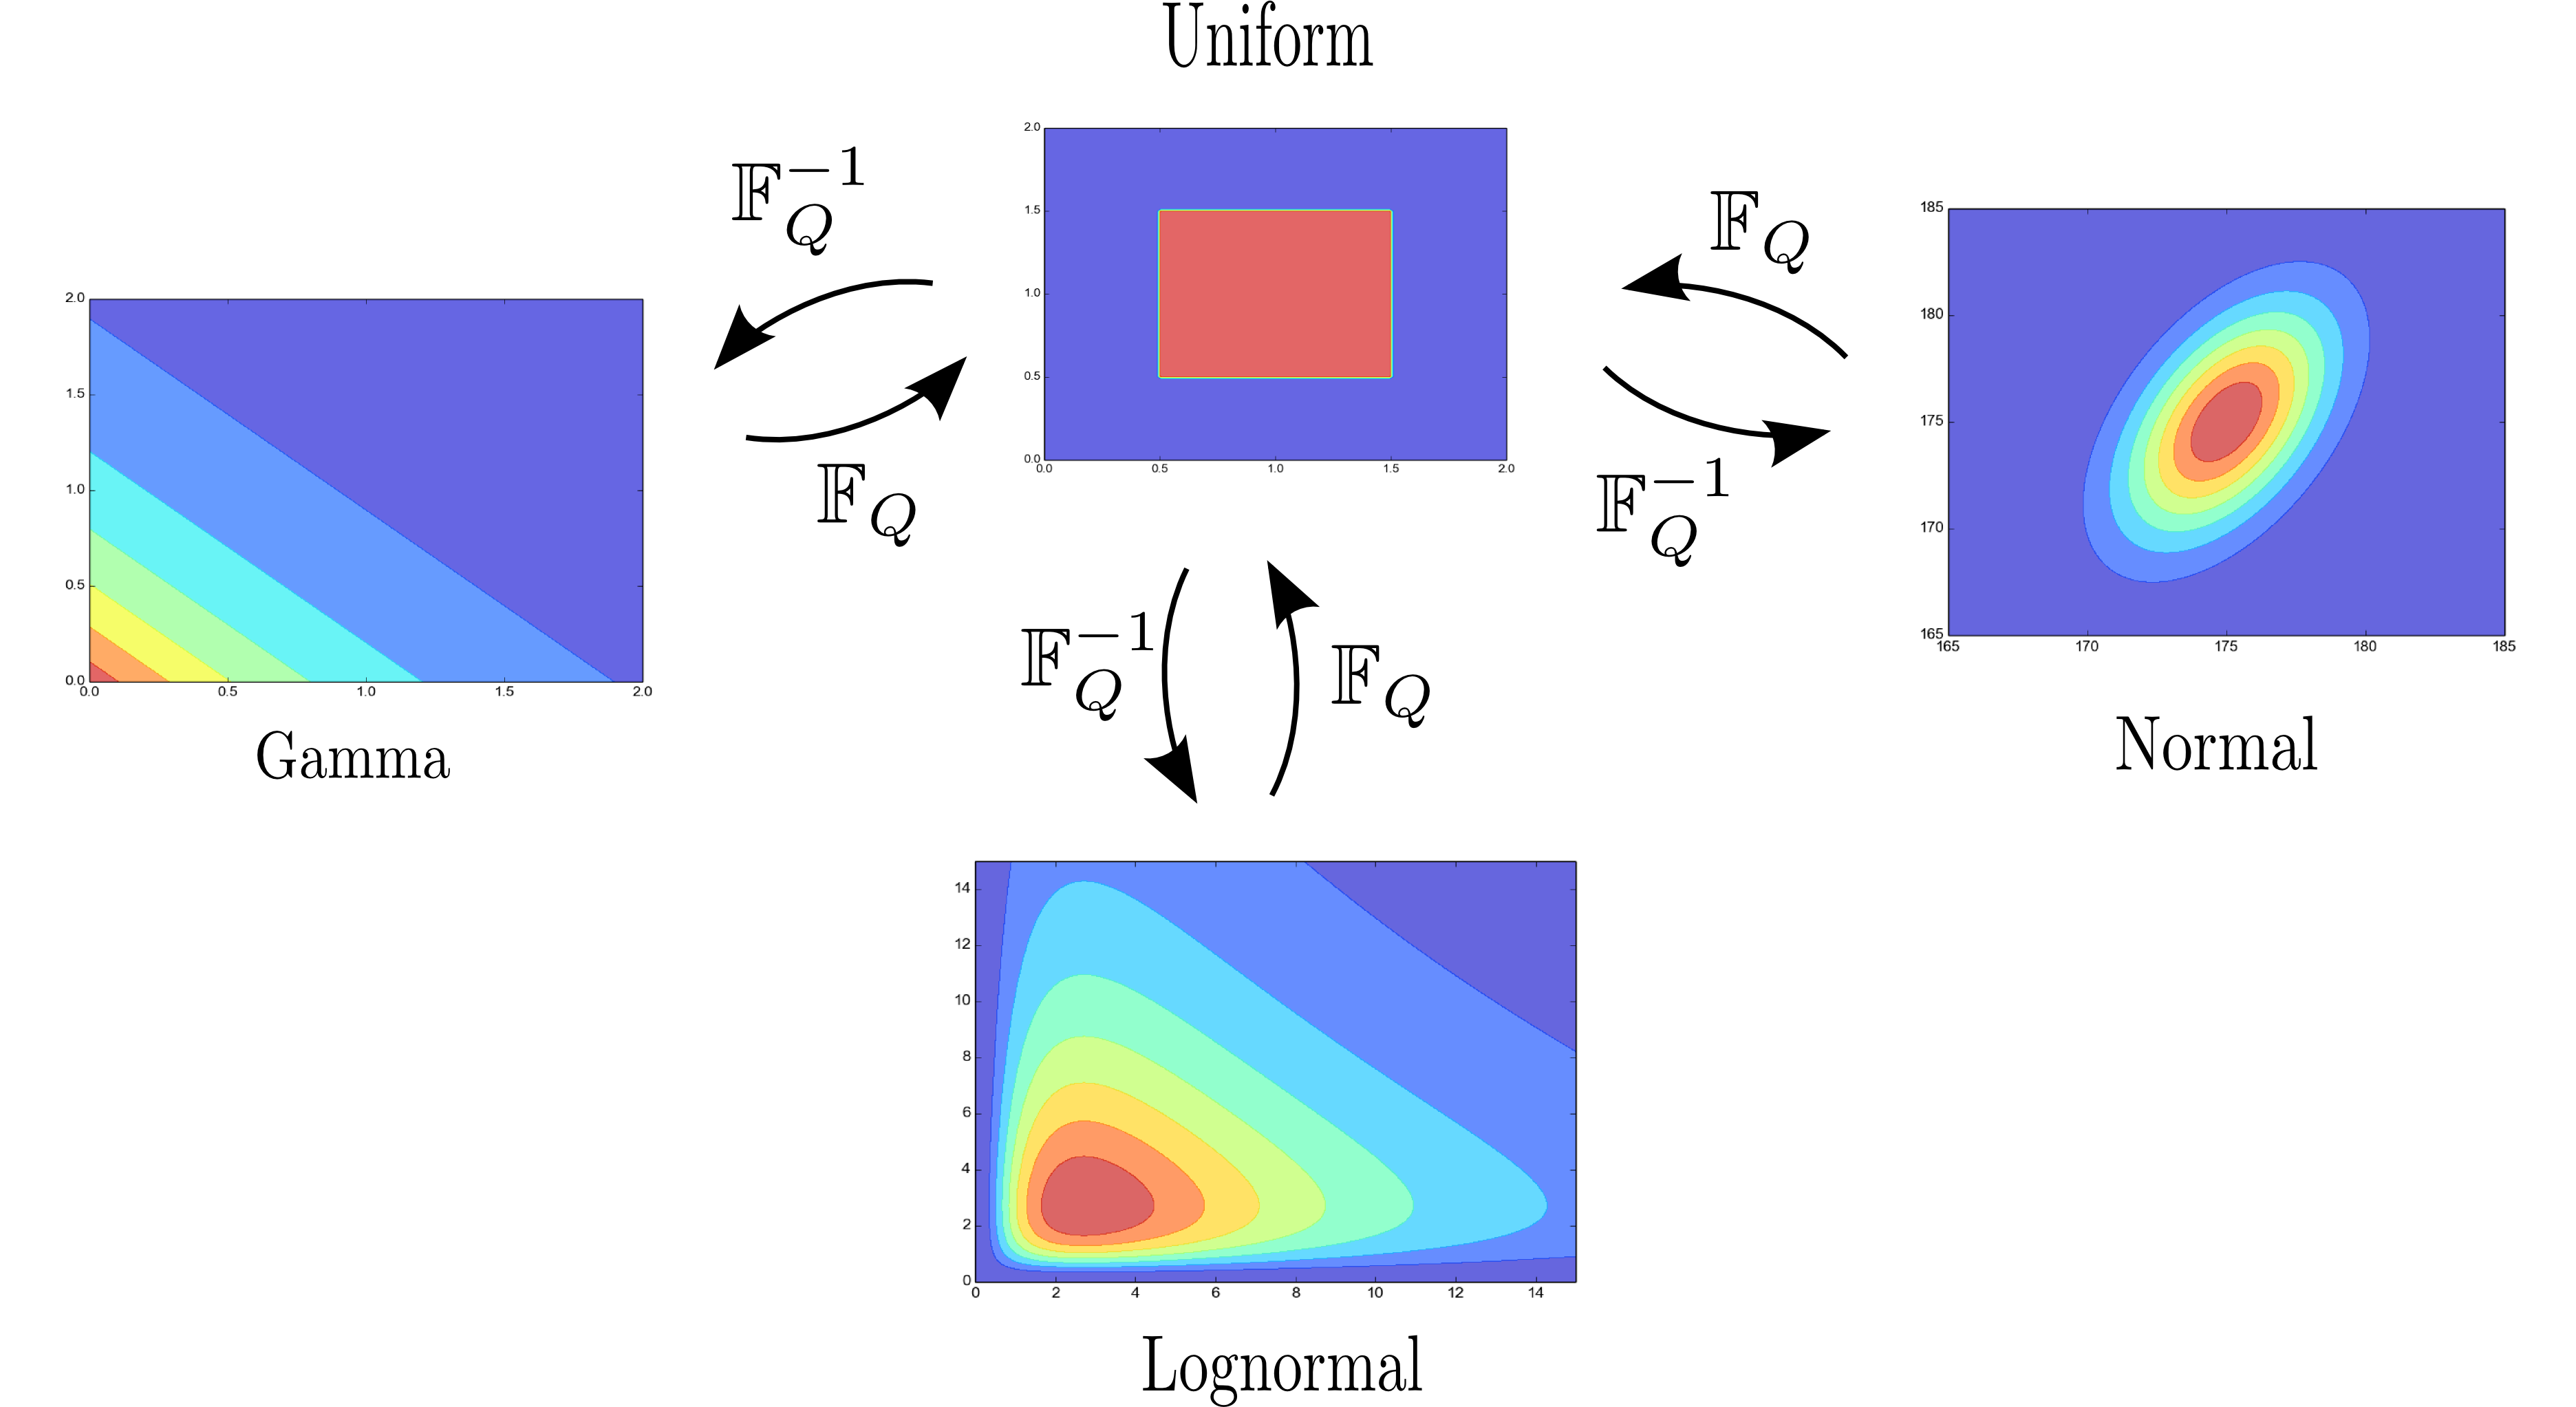
\includegraphics[width = \textwidth]{distributions.png}
 %\end{figure}

 %\end{frame}

 %\begin{frame}
 %\frametitle{Chaospy is built around the Rosenblatt transformation which enables several useful properties}

%\begin{itemize}[<+->]
%\item Sampling of all probability distributions.
%\vspace{3mm}
%\item Quasi-Monte Carlo sampling is available for any probability distribution.
% \vspace{3mm}
% \item Polynomial Chaos expansions are available for any probability distribution, even dependent variables
%\end{itemize}

% \end{frame}



\begin{frame}
  \frametitle{Mapping in probability space; the idea behind Polynomial Chaos (PC) theory is to approximate our forward model with a polynomial}
  \begin{align*}
      u(x; q) & &\approx && \hat u_M(x;q) && =
      && \sum_{n=0}^N && {\color<3>{red}c_n(x)}\quad && {\color<4>{red}P_n(q)}\\
      &&  &&  &&  &&  && {\color<3>{red}\text{Coefficient}} && {\color<4>{red}\text{Polynomial}}
  \end{align*}

$\hat u_M(x; q)$ is the mapping from the uncertain variables $q$ to the response variable $u$, $x$ is a set variable.

% \hspace{10.5mm} $q$ are the uncertain variables
%   \begin{align*}
%       N = \frac{(M + D)!}{M!D!} - 1, \quad D\text{ is the number of dimensions}\\
%   \end{align*}
\pause
\vspace{1cm}
Mean and variance are calculated from $\hat u_M(x;q)$.
\end{frame}



%\begin{frame}
%  \frametitle{Want to have the Best Linear Unbiased Estimator (BLUE)}

%We have the variance criteria

%\[ \Var{|u - \hat u_M|}\]
%\pause

%and want to choose the Best Linear Unbiased Estimator (BLUE):
%\begin{align*}
%    \E{\hat u_M} &= u\\
%    \Var{|u - \hat u_M|} &\leq \Var{|u - \hat u^*|} &    &\forall  u^* \in P_M\\
%    &&& \forall M \in |\mathbb{Z}^+|
%\end{align*}
%    All polynomials $P_n$ and coefficients $c_n$ are free.
%\end{frame}



%\begin{frame}
%    \frametitle{We need to choose Askey-Wilson polynomials}
%Choosing the Best Linear Unbiased Estimator leads to:
%\begin{align*}
%\E{P_nP_m} &= 0  & \forall n \neq m\\
%\end{align*}

%This is fulfilled by choosing Askey-Wilson polynomials, a family of orthogonal polynomials.
%\end{frame}



%
% \begin{frame}
%  \frametitle{The computational essence of Polynomial Chaos}
% \[\hat u_M(x;q) = \sum_{n=0}^N c_n(x) P_n(q)\]
% \vspace{10mm}
%
%  We need to find the orthogonal polynomials $P_n(q)$ and the coefficients $c_n(x)$.
%
% \end{frame}



\begin{chaospy}{$P_n$ are orthogonal polynomials and are generaly calculated through the three-term discretized Stiltjes recursion}
\begin{lstlisting}[language=python]
dist = cp.Normal()

P = cp.orth_ttr(3, dist)
|\pause|
print P
[1.0, q0, q0^2-1.0, q0^3-3.0q0]
\end{lstlisting}
\end{chaospy}


\begin{frame}
  \frametitle{Methods for generating expansions of orthogonal polynomials}
\begin{center}
\def\arraystretch{1.1}

  \begin{tabular}{ll|lll}
Orthogonalization Method	&& Dakota	&Turns &	Chaospy \\\hline
Askey–Wilson scheme &&	Yes	&Yes&	\textbf{\textcolor{green}{Yes}}\\
Bertran recursion &&	No	&No	&\textbf{\textcolor{green}{Yes}}\\
Cholesky decomposition &&	No	&No&	\textbf{\textcolor{green}{Yes}}\\
Discretized Stieltjes &&	Yes	&No&	\textbf{\textcolor{green}{Yes}}\\
Modified Chebyshev &&	Yes	& Yes&	\textbf{\textcolor{red}{No}}\\
Modified Gram–Schmidt &&	Yes &	Yes & \textbf{\textcolor{green}{Yes}}\\
\end{tabular}
\end{center}
\end{frame}





%
% \begin{frame}
%     This leads to
% \begin{align*}
% \E{P_nP_m} &= 0  & \forall n \neq m\\
% c_n &= \frac{\E{uP_n}}{\E{P_n^2}}
% \end{align*}
%
% Solution:
% \begin{align*}
%     \E{P_nP_m} &= 0 & &\text{Fulfilled by choosing orthogonal polynomials} \\
%     c_n &&& \text{Can be approximated by quadrature rules, }\\
%         &&& \text{the probability distribution is used as a weight function}
% \end{align*}
% \end{frame}




%\begin{frame}
%\frametitle{$c_n$ is approximated by quadrature rules, called the pseudo-spectral method}
%    Choosing the Best Linear Unbiased Estimator also leads to:
%
%\begin{align*}
%c_n &= \frac{\E{uP_n}}{\E{P_n^2}}
%\end{align*}
%$c_n$ is approximated by quadrature rules where the probability distribution is used as a weight function.
%\end{frame}



\begin{chaospy}{The pseudo-spectral method, used to calculate $c_n$, needs numerical integration, which demands generating quadrature nodes and weights}
    \scriptsize

\begin{lstlisting}[language=python]
dist = cp.Normal()

nodes, weights = cp.generate_quadrature(2, dist, rule="G")
|\pause|
print nodes
[[-1.73205081  0.          1.73205081]]
print weights
[ 0.16666667  0.66666667  0.16666667]
\end{lstlisting}
\normalsize

\end{chaospy}


\begin{frame}
  \frametitle{Numerical integration strategies implemented in the three software toolboxes}

\begin{center}
\newcolumntype{g}{>{\columncolor{gray}}l}
\def\arraystretch{1.1}
  \begin{tabular}{ll|lll}
Node and weight generators&&	Dakota	&Turns&	Chaospy\\\hline
Clenshaw-Curtis quadrature &&	Yes&	No	&\textbf{\textcolor{green}{Yes}}\\
Cubature rules &&	Yes	&No&	\textbf{\textcolor{red}{No}}\\
Gauss-Legendre quadrature &&	Yes	&No&	\textbf{\textcolor{green}{Yes}}\\
Gauss-Patterson quadrature &&	Yes	&No&	\textbf{\textcolor{green}{Yes}}\\
Genz-Keister quadrature &&	Yes	&No&	\textbf{\textcolor{green}{Yes}}\\
Leja quadrature &&	No&	No&	\textbf{\textcolor{green}{Yes}}\\
Monte Carlo integration &&	Yes&	No	&\textbf{\textcolor{green}{Yes}}\\
Optimal Gaussian quadrature &&	Yes&	No&	\textbf{\textcolor{green}{Yes}}\\
\end{tabular}
\end{center}
\end{frame}


\begin{chaospy}{One slide is enough for the full implementation with the pseudo-spectral method
    in Chaospy}
    \scriptsize
%  def u(x, a, I):
%    return I*np.exp(-a*x)
%  |\pause|
 \begin{lstlisting}[language=python]
dist_a = cp.Uniform(0, 0.1)
dist_I = cp.Uniform(8, 10)
dist = cp.J(dist_a,dist_I)
|\pause|
P = cp.orth_ttr(2, dist)
|\pause|
nodes, weights = cp.generate_quadrature(3, dist)
|\pause|
samples_u = [solver(*node) for node in nodes.T]
|\pause|
u_hat = cp.fit_quadrature(P, nodes, weights, samples_u
                          rule="Gaussian")
|\pause|
mean = cp.E(u_hat, dist)
var = cp.Var(u_hat, dist)
\end{lstlisting}
\end{chaospy}


\begin{frame}
 \frametitle{Convergence of polynomial chaos is much faster than the Monte Carlo methods}
\vspace{-5.8mm}
\begin{figure}
    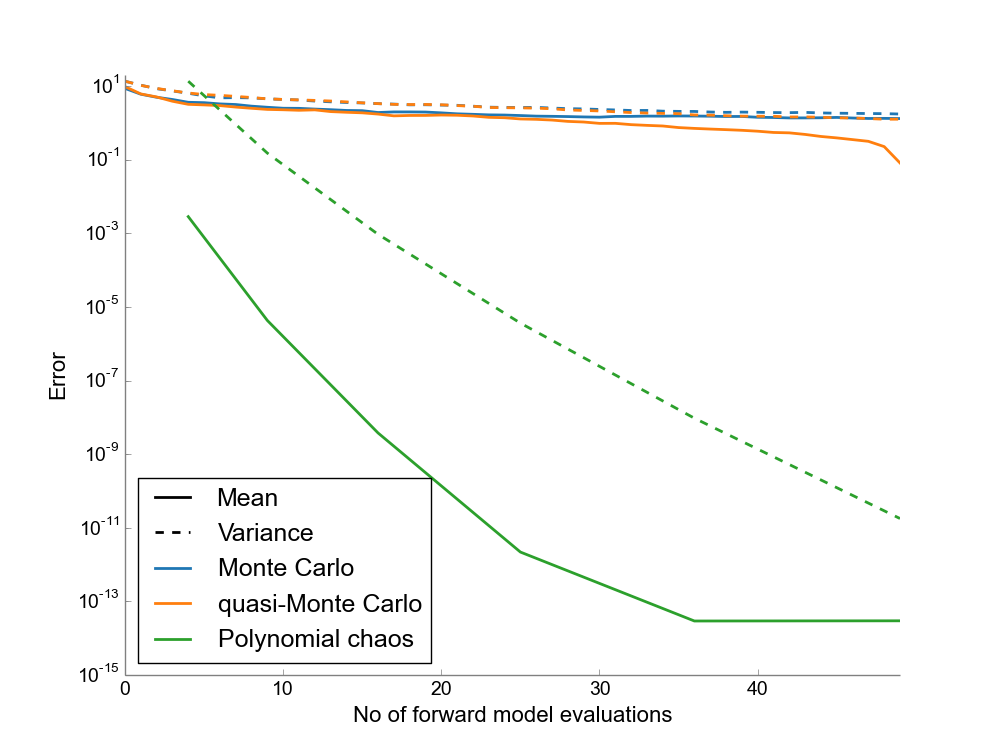
\includegraphics[width=1\textwidth]{qMC-MC-PC_convergence_2D.png}
  \end{figure}

 \end{frame}



%\begin{frame}
% \frametitle{Chaospy can be used for vastly more complicated problems, for example bloodflow simulations}
%
%\vspace{-5.8mm}
%
%  \begin{columns}
%        \column{.5\textwidth}
%        \begin{center}
%    \includegraphics[width=.6\textwidth]{arterialHumanPicture.png}
%        \end{center}
%        \column{.5\textwidth}
%        \begin{center}
%    \includegraphics[width=.6\textwidth]{arterialTreeMascot3D.png}
%        \end{center}
%    \end{columns}
%
%\vspace{5mm}
%\tiny
%Eck V, Feinberg J, Langtangen H, Hellevik L. Stochastic sensitivity analysis for timing and amplitude of pressure waves in the arterial system. Int J Numer Meth Biomed Engng. 2015;31(4):n/a-n/a. doi:10.1002/cnm.2711.
%
 %\end{frame}


\begin{chaospy}{Chaospy is an ideal tool for research in UQ for the statistics expert}

With a few lines of Python code it is easy to customize:
\begin{itemize}[<+->]
    \setlength{\itemsep}{5pt}
    \item distributions
    \item polynomials
    \item integration schemes
    \item sampling schemes
    \item statistical analysis of the result
\end{itemize}

\pause
\vspace{5mm}
Custom polynomials:
    \scriptsize
 \begin{lstlisting}[language=python]
q0, q1 = cp.variable(2)
|\pause|
phi = cp.Poly([1, q0, q1, q0**2 - 1, q0*q1])
|\pause|
print phi
[1, q0, q1, q0^2-1, q0q1]
\end{lstlisting}
\end{chaospy}





 \begin{frame}
 \frametitle{Chaospy handles Polynomial Chaos expansions with stochastically dependent variables}

Diffusion in layered media with uncertain boundary, $l$, and uncertain diffusion constants, $D_0$, $D_1$.

 \begin{figure}
 \includegraphics[height = 0.4\textheight]{layered_media.png}
 \end{figure}

Uncertain $l$ slows down convergence, but introduction of auxiliary \emph{dependent} variables restores convergence.


% Standard polynomial chaos does not work very well, but we can transform our variables to get around the problem.
% The variables then become dependent.

%\pause
%Dependent variables break the orthogonality properties of the polynomials.

%\pause
%Chaospy uses Rosenblatt transformations to solve this problem.

\end{frame}


%\begin{chaospy}{Chaospy handles Polynomial Chaos expansions with stochastically dependent variables}
%  \scriptsize
%\begin{lstlisting}[language=Python]
%
%C = [[1,0.5],[0.5,1]]
%mu = np.array([0, 0])
%dist_Q = cp.MvNormal(mu, C)|\pause|
%dist_R = cp.J(cp.Normal(), cp.Normal())
%
%P = cp.orth_ttr(M, dist_R)|\pause|
%nodes_R, weights_R = cp.generate_quadrature(M+1, dist_R)|\pause|
%nodes_Q = dist_Q.inv(dist_R.fwd(nodes_R))|\pause|
%weights_Q = weights_R*\
%    dist_Q.pdf(nodes_Q)/dist_R.pdf(nodes_R)
%|\pause|
%samples_u = [solver(*node) for node in nodes_Q.T]|\pause|
%u_hat = cp.fit_quadrature(P, nodes_R, weights_Q, samples_u)
%\end{lstlisting}
%\end{chaospy}



%\begin{chaospy}{The polynomial approximation can be used as a surrogate model, which allows for computationally cheap statistical analysis}
%    \scriptsize
% \begin{lstlisting}[language=python]
%u_hat = cp.fit_quadrature(P, nodes, weights, solves)
%|\pause|
%samples_q = dist.sample(10**6)
%samples_u = u_hat(*samples_q)
%|\pause|
%mean = np.mean(samples_u, 1)
%var = np.var(samples_u, 1)
%\end{lstlisting}
%\end{chaospy}



%
% \begin{frame}{Advantages and disadvantages of Chaospy}{}
% \onslide<1->\bf \color{green} {Advantages}
% \begin{itemize}
% \onslide<3->\gooditem The programming syntax resembles the mathematics
% \onslide<1->\gooditem Modular software design
% \onslide<5->\gooditem Supports both Monte Carlo and Polynomial Chaos
% \onslide<6->\gooditem Handles dependent variables
% \end{itemize}
% \vspace{8mm}
% \onslide<1->\bf\color{red} Disadvantages
% \begin{itemize}
% \onslide<2->\baditem No gui
% \onslide<4->\baditem The programming syntax lies close to the mathematical theory
% \onslide<7->\baditem Slow
% \end{itemize}
%
% \end{frame}





% \begin{frame}
%  \frametitle{Some random variables are dependent}
%  \begin{figure}
%  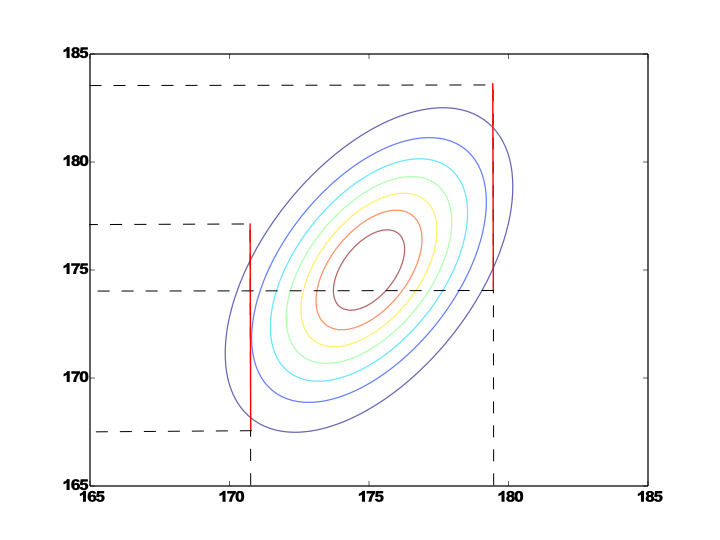
\includegraphics[width = 0.9\textwidth]{dependent.png}
%  \end{figure}
%
%  \end{frame}


%
% \begin{frame}{Transformations manipulates probability distributions}
% \begin{figure}
%  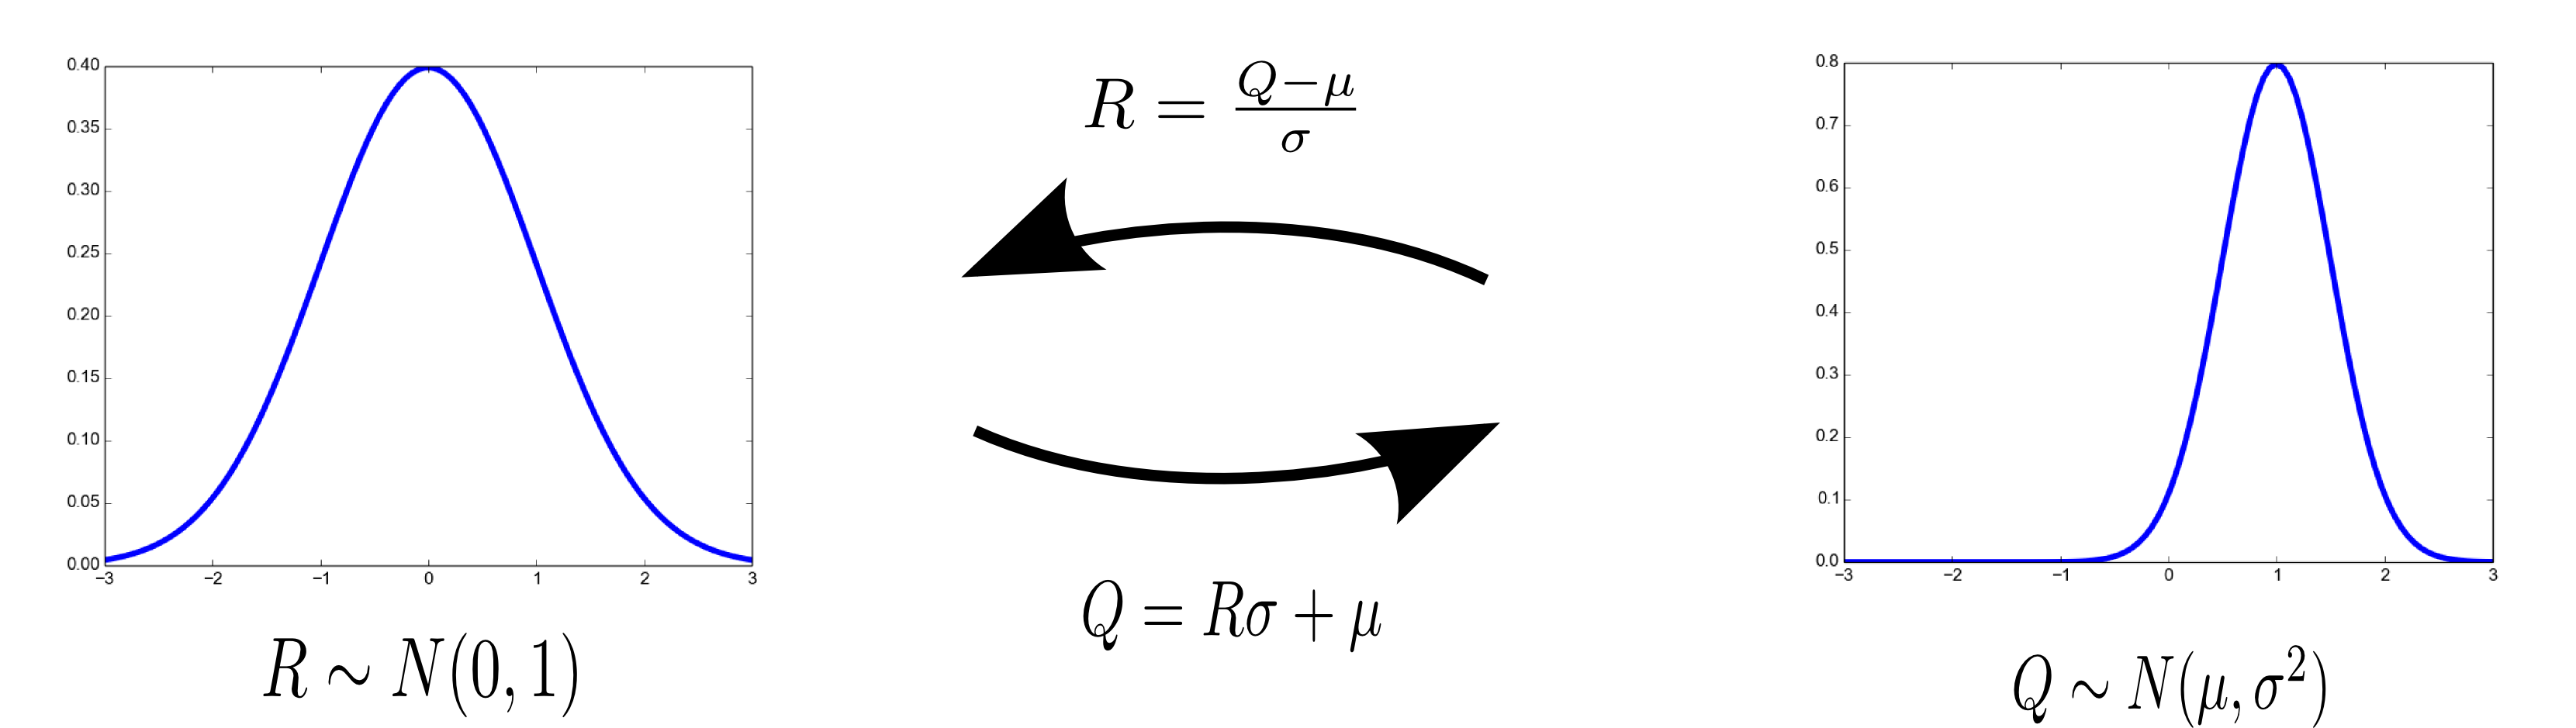
\includegraphics[width=\textwidth]{trans2.png}
% \end{figure}
% \end{frame}




%
% \begin{frame}
%  \frametitle{Dependent variables break the orthogonality property of Polynomal Chaos!}
%  \scriptsize
%  \[  P_{\mathfrak i} = P_{i_1}^{(1)}P_{i_2}^{(2)}\cdots P_{i_D}^{(D)} \qquad \mathfrak i = (i_1,i_2,...,i_D)\]
%  \pause
%  \begin{align*}
%      \inner{ P_\mathfrak{i},P_\mathfrak{j}} &= E(P_\mathfrak{i},P_\mathfrak{j})\\
%   \onslide<3-> {&=\E{P_{i_1}^{(1)}\cdots P_{i_D}^{(D)}P_{j_1}^{(1)}\cdots P_{j_D}^{(D)}}}\\
%   \onslide<4-> {&=\E{P_{i_1}^{(1)}P_{j_1}^{(1)}}\cdots \E{P_{i_D}^{(D)}P_{j_D}^{(D)}}}\\
%   \onslide<5-> {&=\dots}\\
%   \onslide<5-> {&=\norm{P_{\mathfrak{i}}^{(1)}}\delta_{\mathfrak{i}\mathfrak{j}}}
%  \end{align*}
%  \onslide<6->
% \begin{alert}{But the problem is:}
% \[\E{uv} \neq \E{u}\E{v} \qquad \text{when $u$ and $v$ are
% stochastically dependent}\]
%  \end{alert}
%  \end{frame}






%  \begin{chaospy}{Point collocation with Rosenblatt transformation}
%  \scriptsize
%  \begin{lstlisting}[language=Python]
% def u(x,a, I):
%     return I*np.exp(-a*x)
% |\pause|
% dist_R = cp.J(cp.Normal(), cp.Normal())
% C = [[1, 0.5], [0.5, 1]]
% mu = [0, 0]
% dist_Q = cp.MvNormal(mu, C)
% |\pause|
% P = cp.orth_ttr(M, dist_R)|\pause|
% nodes_R = dist_R.sample(2*len(P), "M")|\pause|
% nodes_Q = dist_Q.inv(dist_R.fwd(nodes_R))
% |\pause|
% x = np.linspace(0, 1, 100)
% samples_u = [u(x, *node) for node in nodes_Q.T]|\pause|
% u_hat = cp.fit_regression(P, nodes_R, samples_u)
% \end{lstlisting}
% \end{chaospy}




\begin{frame}{Summary: Chaospy is a Python toolbox for forward model UQ with advanced Monte Carlo methods and Polynomial Chaos expansions}
\vspace{-5mm}
\begin{columns}

     \column{.5\textwidth}
     \begin{center}
      \bf{Chaospy is modular, flexible, with syntax that resembles the mathematics}
     \end{center}
     \column{.5\textwidth}
     \begin{center}
            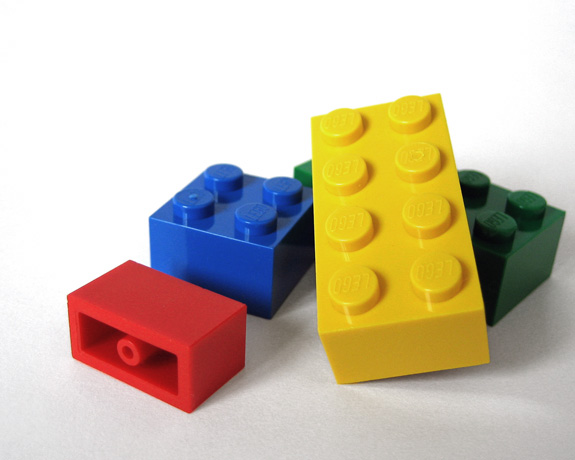
\includegraphics[width=0.6\textwidth]{lego.jpg}
     \end{center}

 \end{columns}

\vspace{10mm}

\begin{columns}
  \column{.5\textwidth}
  \begin{center}
   \bf{A vast collection of methods, ideal for method comparisons}
  \end{center}
       \column{.5\textwidth}
     \begin{center}
            \includegraphics[width=0.6\textwidth]{bookshelf.jpg}
     \end{center}

 \end{columns}

%\begin{tikzpicture}[remember picture, overlay, font=\sffamily]
%    \node [align=left, xshift=0.3\textwidth,yshift=0.1\textwidth] (image1) at (current page.center)
%          {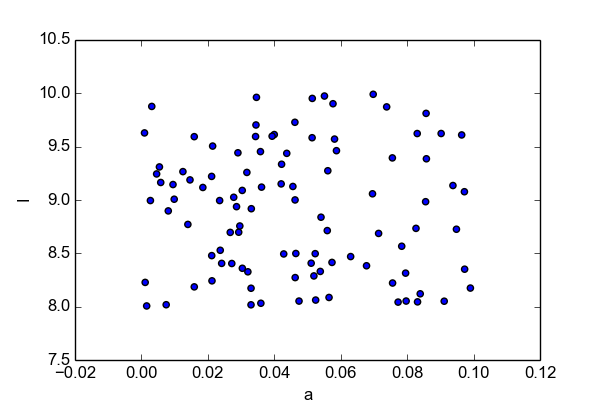
\includegraphics[width = 0.3\textwidth]{samples.png}};
%    \node[align=left] at (image1.west) {\hspace{-7cm} \bf Advanced Monte Carlo methods};
%  \end{tikzpicture}


%\begin{tikzpicture}[remember picture, overlay, font=\sffamily]
%    \node [align=left, xshift=0.3\textwidth,yshift=-0.15\textwidth] (image2) at (current page.center)
%          {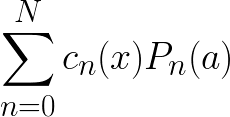
\includegraphics[width = 0.25\textwidth]{pc.png}};
%    \node[align=left] at (image2.west) {\hspace{-7.95cm} \bf Polynomial Chaos expansions};
%  \end{tikzpicture}



  % \begin{tikzpicture}[remember picture, overlay, font=\sffamily]
  %     \node [align=left, xshift=0.49\textwidth,yshift=-0.37\textwidth] (image2) at (current page.center)
  %           {
\includegraphics[width = 0.35\textwidth]{cinpla.png}};
  %   \end{tikzpicture}
  %
  %   \begin{tikzpicture}[remember picture, overlay, font=\sffamily]
  %       \node [align=left, xshift=-0.45\textwidth,yshift=-0.37\textwidth] (image2) at (current page.center)
  %             {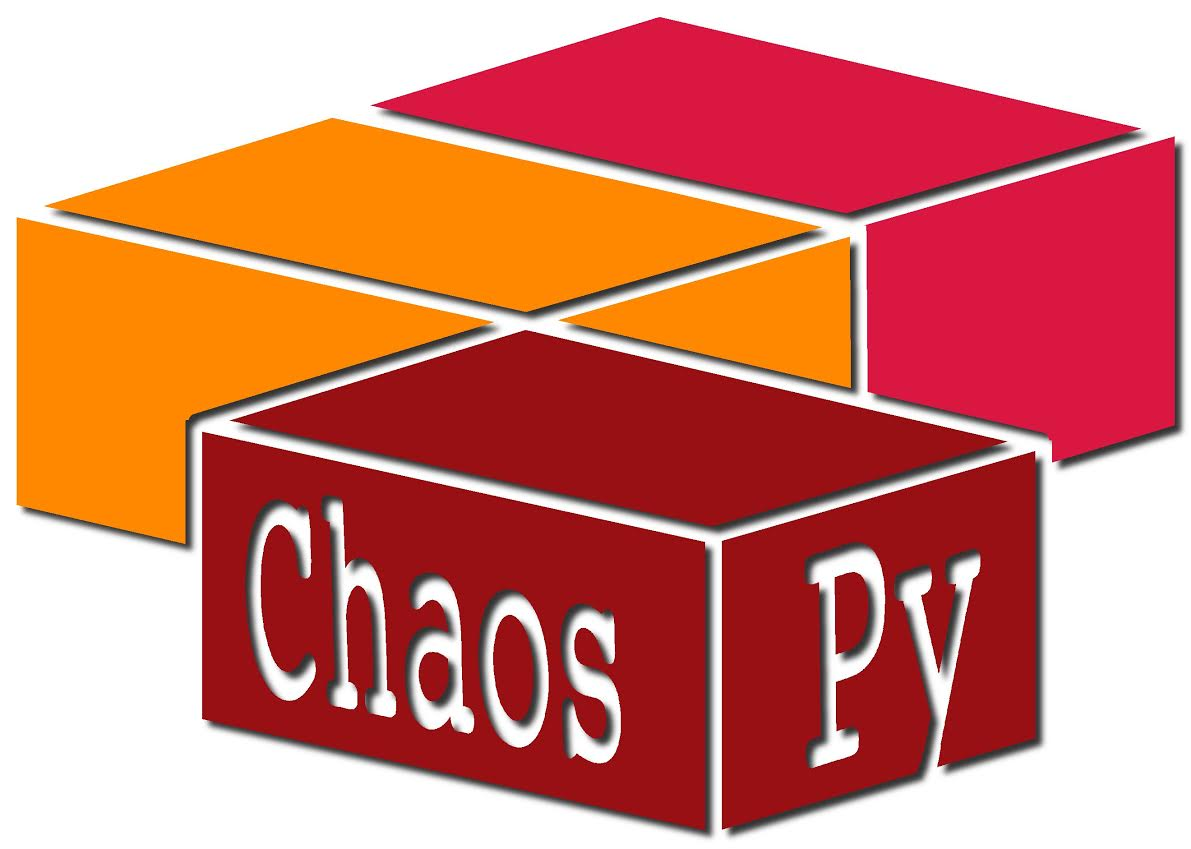
\includegraphics[width = 0.18\textwidth]{chaospy_logo.jpg}};
  %     \end{tikzpicture}

% \pause
% \begin{tikzpicture}[remember picture, overlay, font=\sffamily]
%
%   \node[align=left, yshift=0.1\textwidth] at (current page.south){ \bf Questions?};
% \end{tikzpicture}
%
% \vspace{3.5cm}
%
%   \begin{alert}{Installation instructions:}\\
%   \scriptsize
%       \href{https://github.com/hplgit/chaospy}{https://github.com/hplgit/chaospy}\\
% %\verb;http://github.com/hplgit/chaospy/;
%   \end{alert}
%
%
%
%   \begin{alert}{References:}\\
%   \scriptsize
%       Feinberg, J., \& Langtangen, H. (2015). Chaospy: An open source tool for designing methods of uncertainty quantification. Journal Of Computational Science, 11, 46-57\\
%       \href{http://www.sciencedirect.com/science/article/pii/S1877750315300119}{http://www.sciencedirect.com/science/article/pii/S1877750315300119}
%   \end{alert}



\end{frame}


  \begin{frame}{Summary: Chaospy is a Python toolbox for forward model UQ with advanced Monte Carlo methods and Polynomial Chaos expansions}
  \begin{alert}{Installation instructions:}\\
  \scriptsize
      \href{https://github.com/hplgit/chaospy}{https://github.com/hplgit/chaospy}\\
%\verb;http://github.com/hplgit/chaospy/;
  \end{alert}


\vspace{7mm}

  \begin{alert}{Reference:}\\
  \scriptsize
      Feinberg, J., \& Langtangen, H. P. (2015). Chaospy: An open source tool for designing methods of uncertainty quantification. Journal Of Computational Science, 11, 46-57\\

      \vspace{3mm}
      \href{http://hplgit.github.io/chaospy/doc/pub/chaospy-4screen.pdf}{http://hplgit.github.io/chaospy/doc/pub/chaospy-4screen.pdf}
  \end{alert}

  \begin{tikzpicture}[remember picture, overlay, font=\sffamily]
      \node [align=left, xshift=0.49\textwidth,yshift=-0.37\textwidth] (image2) at (current page.center)
            {
\includegraphics[width = 0.35\textwidth]{cinpla.png}};
    \end{tikzpicture}

    \begin{tikzpicture}[remember picture, overlay, font=\sffamily]
        \node [align=left, xshift=-0.45\textwidth,yshift=-0.37\textwidth] (image2) at (current page.center)
              {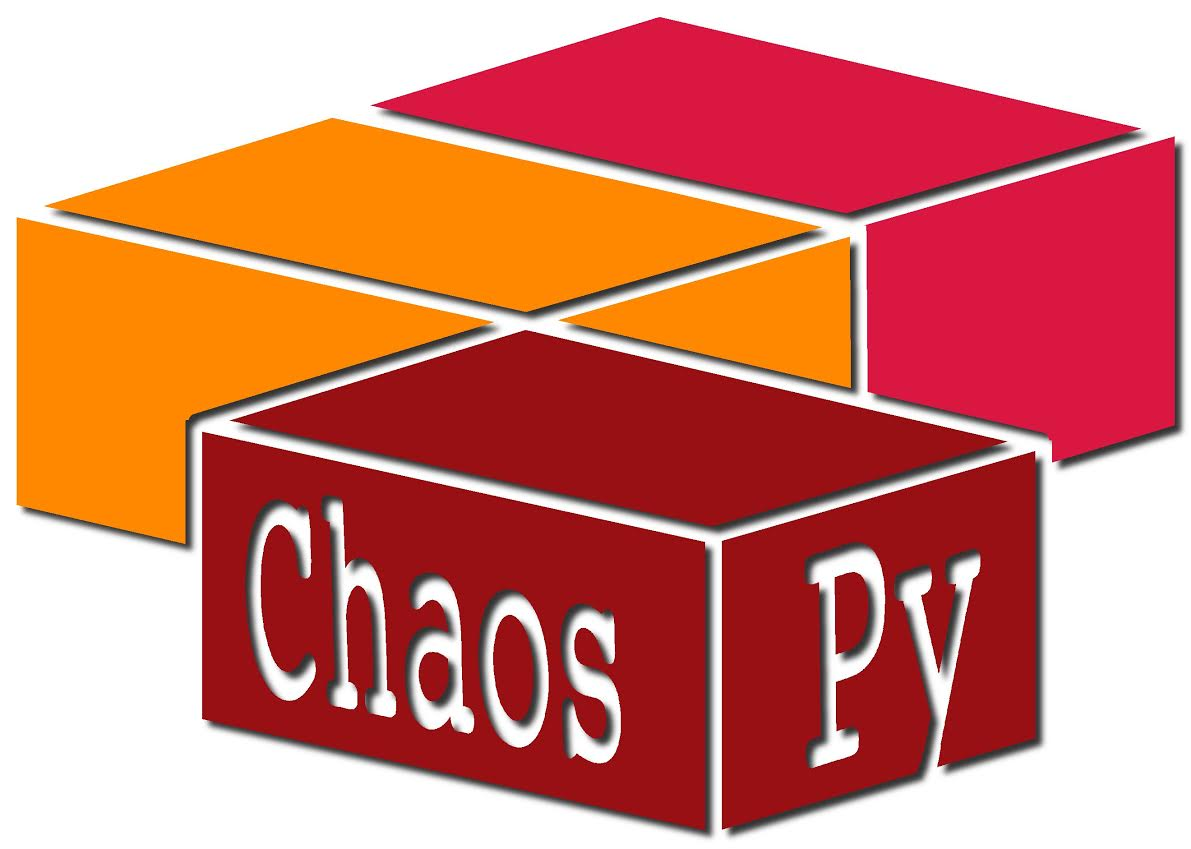
\includegraphics[width = 0.18\textwidth]{chaospy_logo.jpg}};
      \end{tikzpicture}

\pause
\begin{tikzpicture}[remember picture, overlay, font=\sffamily]

  \node[align=left, yshift=0.15\textwidth] at (current page.south){ \bf \large Questions?};
\end{tikzpicture}



\end{frame}


\end{document}
